\subsection{OLCF and Titan}

In 2004, the Oak Ridge Leadership Computing Facility (OLCF) was established at
Oak Ridge National Laboratory (ORNL). The OLCF's mission is to accelerate
scientific discovery and engineering progress by providing outstanding computing
and data management resources to high-priority research and development
projects. Among other resources, OLCF manages Titan, a leadership-class and the
fastest open-science supercomputer in the US. Titan enables scientists to
evaluate and assess various complex physical phenomena via large-scale
computational simulations.

Titan is a Cray XK7 system with 18,688 compute nodes~\cite{top500}. Each compute
node is equipped with an AMD Opteron CPU and a Nvidia Tesla GPU. This hybrid
design provides improved energy efficiency, as well as an order of magnitude in
computational capacity over its predecessor. Titan has 710 TB of total system
memory and a center-wide parallel file system known as Spider II~\cite{spider2}.
Spider II is one of the world's fastest and largest POSIX complaint parallel
file systems, designed to serve write-heavy I/O workloads generated by Titan
compute clients and other OLCF resources.


% The topology and architecture details of Spider II infrastructure are
% illustrated in Figure~\ref{fig:xk7-compute-node} and
% described as follows:
%
%
% \begin{figure}[!htb]
%     \centering
%     \begin{tabular}{cc}
%         {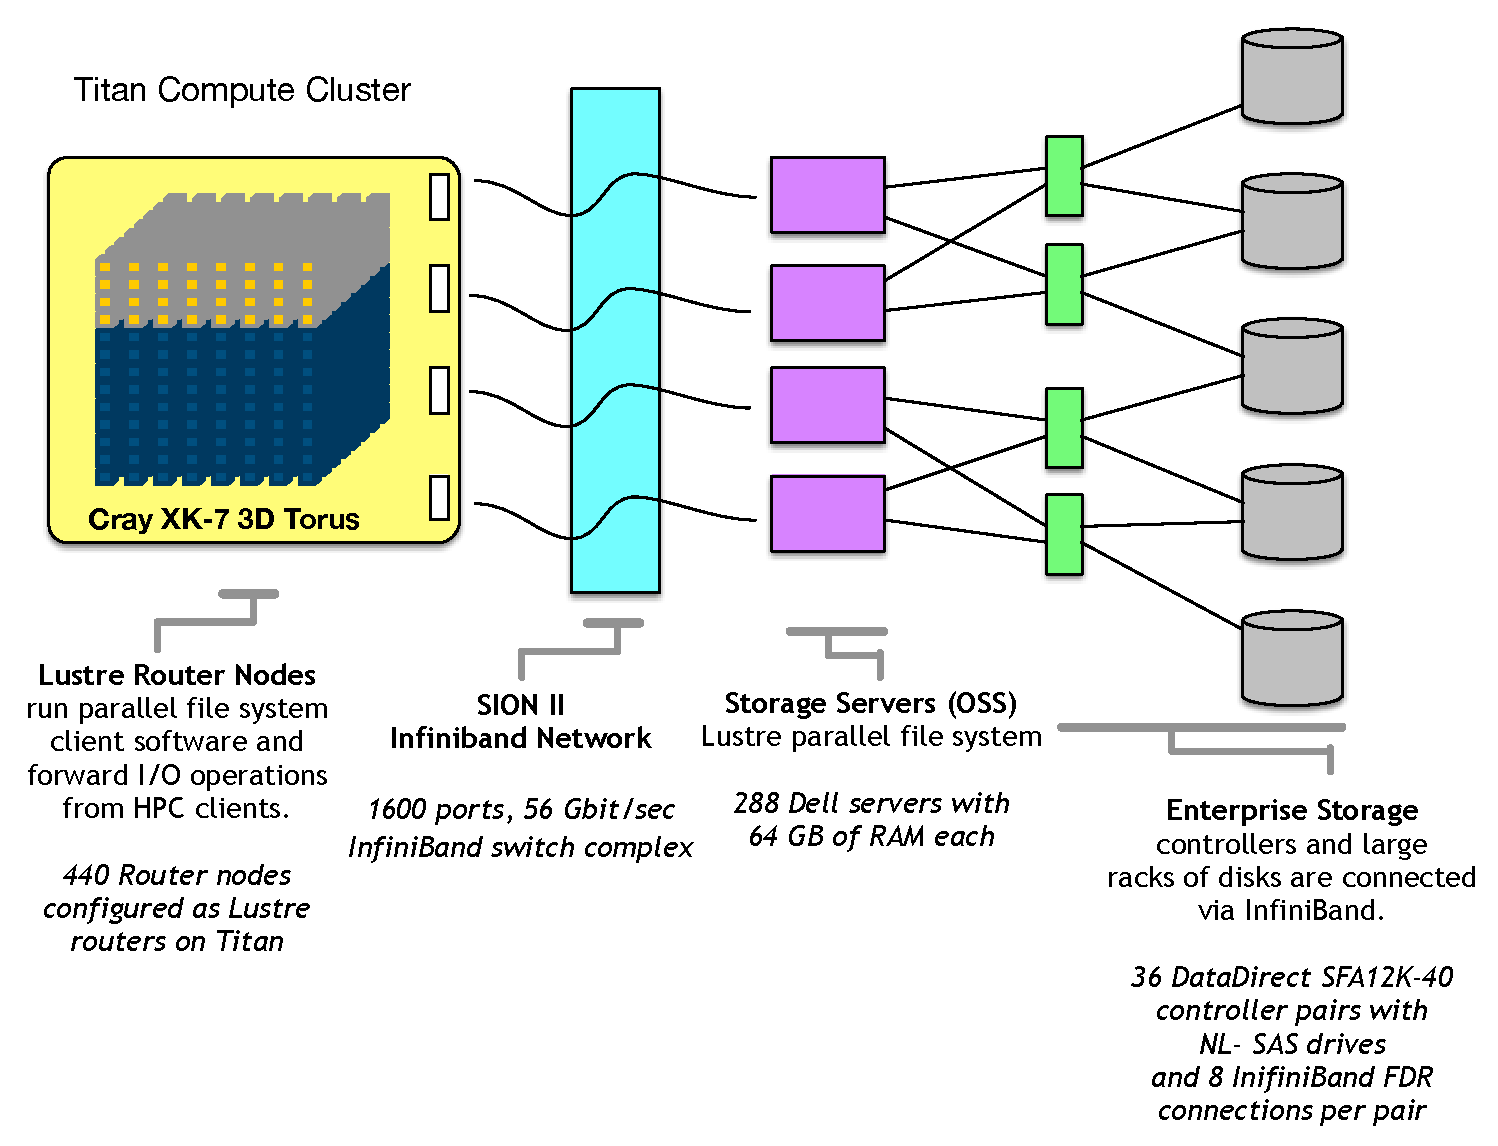
\includegraphics[width=0.48\textwidth]{figures/spider2arch.pdf}}\\
%     \end{tabular}
%     \caption{Infrastructure and I/O path between Titan (Cray XK7) and its backend storage}
%     \label{fig:xk7-compute-node}
% \end{figure}
%
%
%
% Spider II is based on the Lustre technology~\cite{lustre}.  It is configured
% and deployed as two independent, non-overlapping file systems, each with 144
% Lustre Object Storage Servers (OSSs) and 1,008 Lustre Object Storage Targets
% (OSTs). Spider II offers ~30 PB usable file system capacity to OLCF systems and
% users and has over 1 TB/s aggregate write I/O performance.
